\documentclass[,a4paper,12pt,french]{article}

\usepackage{../../../../Style}

\geometry{margin=10mm}
\setlist[itemize]{align=parleft,left=5pt..15pt}
\setlist[enumerate]{align=parleft,left=5pt..20pt}

\usepackage{tikz-3dplot}
\usetikzlibrary{decorations.pathreplacing,calligraphy}
\definecolor{boite}{RGB}{247,197,57}

\titlespacing*{\section}{-5mm}{5mm}{1mm}

\pagestyle{empty}

% Début du document
%%%%%%%%%%%%%%%%%%%
\begin{document}

\titre{La boite}

\section*{Quelques exemples}

\begin{minipage}{0.325\linewidth}
\begin{center}
 \tdplotsetmaincoords{70}{60}
   \begin{tikzpicture}[scale=1,line cap=butt,line join=round,tdplot_main_coords,declare function={a=3.6;b=3.6;h=0.45;k=0;
   }] 
    \begin{scope}[canvas is yx plane at z=0]
    \path
    (0,0) coordinate (A) 
     (a,0) coordinate (B)
      (a,b) coordinate (C)
      (0,b) coordinate (D);
    \end{scope}
    \begin{scope}[canvas is yx plane at z=h]
 \path
 (0,k) coordinate (A') 
 (a,k) coordinate (B')
 (a,b+k) coordinate (C')
 (0,b+k) coordinate (D');
 \end{scope}  
 \begin{scope}[opacity=1,thick]
\draw[fill=black!10!boite, dotted] (A) --(B)  -- (C) -- (D) -- cycle;
\draw[fill=black!10!boite, dotted] (A) --(B)  -- (B') -- (A') -- cycle;
\draw[fill=boite, dotted] (B) --(C)  -- (C') -- (B') -- cycle;
\draw[fill=black!5!boite] (C) --(D)  -- (D') -- (C') -- cycle;
\draw[fill=white!10!boite] (A) --(D)  -- (D') -- (A') --cycle;
\draw (A') --(B')  -- (C') -- (D') --cycle;
\end{scope}
\end{tikzpicture}

\vspace{2mm}

\begin{minipage}{\linewidth}
Hauteur: 1 cm

Longueur et largeur: 8 cm

Volume: $8 \times 8 \times 1 = 64$ cm$^3$
\end{minipage}
\end{center}
\end{minipage}
\begin{minipage}{0.325\linewidth}
\begin{center}
 \tdplotsetmaincoords{70}{60}
   \begin{tikzpicture}[scale=1,line cap=butt,line join=round,tdplot_main_coords,declare function={a=2.7;b=2.7;h=0.9;k=0;
   }] 
    \begin{scope}[canvas is yx plane at z=0]
    \path
    (0,0) coordinate (A) 
     (a,0) coordinate (B)
      (a,b) coordinate (C)
      (0,b) coordinate (D);
    \end{scope}
    \begin{scope}[canvas is yx plane at z=h]
 \path
 (0,k) coordinate (A') 
 (a,k) coordinate (B')
 (a,b+k) coordinate (C')
 (0,b+k) coordinate (D');
 \end{scope}  
 \begin{scope}[opacity=1,thick]
\draw[fill=black!10!boite, dotted] (A) --(B)  -- (C) -- (D) -- cycle;
\draw[fill=black!10!boite, dotted] (A) --(B)  -- (B') -- (A') -- cycle;
\draw[fill=boite, dotted] (B) --(C)  -- (C') -- (B') -- cycle;
\draw[fill=black!5!boite] (C) --(D)  -- (D') -- (C') -- cycle;
\draw[fill=white!10!boite] (A) --(D)  -- (D') -- (A') --cycle;
\draw (A') --(B')  -- (C') -- (D') --cycle;
\end{scope}
\end{tikzpicture}
\vspace{2mm}

\begin{minipage}{\linewidth}
Hauteur: 2 cm

Longueur et largeur: 6 cm

Volume: $6 \times 6 \times 2 = 72$ cm$^3$
\end{minipage}
\end{center}
\end{minipage}
\begin{minipage}{0.325\linewidth}
\begin{center}
 \tdplotsetmaincoords{70}{60}
   \begin{tikzpicture}[scale=1,line cap=butt,line join=round,tdplot_main_coords,declare function={a=1.8;b=1.8;h=1.35;k=0;
   }] 
    \begin{scope}[canvas is yx plane at z=0]
    \path
    (0,0) coordinate (A) 
     (a,0) coordinate (B)
      (a,b) coordinate (C)
      (0,b) coordinate (D);
    \end{scope}
    \begin{scope}[canvas is yx plane at z=h]
 \path
 (0,k) coordinate (A') 
 (a,k) coordinate (B')
 (a,b+k) coordinate (C')
 (0,b+k) coordinate (D');
 \end{scope}  
 \begin{scope}[opacity=1,thick]
\draw[fill=black!10!boite, dotted] (A) --(B)  -- (C) -- (D) -- cycle;
\draw[fill=black!10!boite, dotted] (A) --(B)  -- (B') -- (A') -- cycle;
\draw[fill=boite, dotted] (B) --(C)  -- (C') -- (B') -- cycle;
\draw[fill=black!5!boite] (C) --(D)  -- (D') -- (C') -- cycle;
\draw[fill=white!10!boite] (A) --(D)  -- (D') -- (A') --cycle;
\draw (A') --(B')  -- (C') -- (D') --cycle;
\end{scope}
\end{tikzpicture}
\vspace{2mm}

\begin{minipage}{\linewidth}
Hauteur: 3 cm

Longueur et largeur: 4 cm

Volume: $4 \times 4 \times 3 = 48$ cm$^3$
\end{minipage}
\end{center}
\end{minipage}

\vspace{2mm}

Nous pourrions faire une multitude de tests pour nous approcher de la valeur donnant un volume maximal, mais ce serait long...

\section*{Introduction d'une inconnue}

\compo[0.43]
{
\begin{centrer}
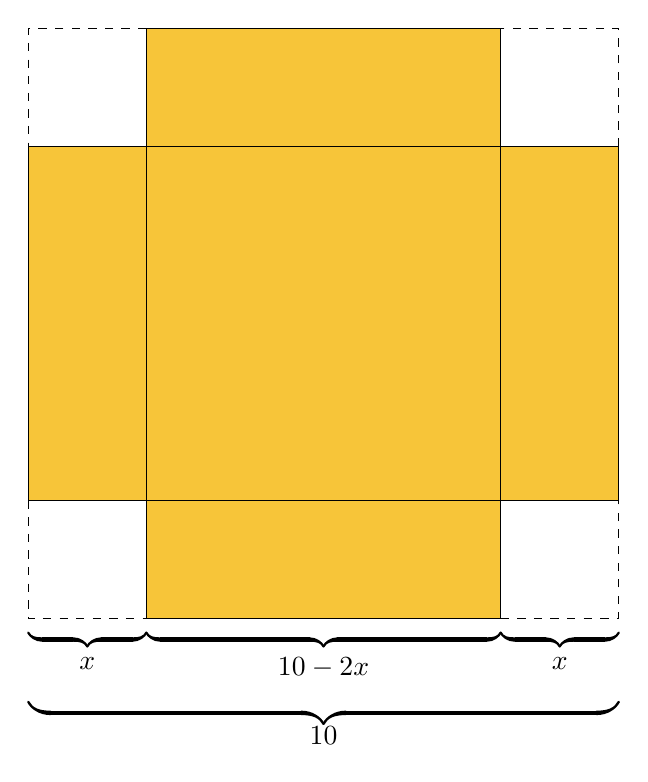
\begin{tikzpicture}[scale=0.75]
\draw[fill=boite] (2,2) -- (10,2) -- (10,8) -- (0,8) -- (0,2) -- (2,2) -- (2,0) -- (8,0) -- (8,10) -- (2,10) -- cycle;
\draw[dashed] (0,2) -- (0,0) -- (2,0);
\draw[dashed] (8,0) -- (10,0) -- (10,2);
\draw[dashed] (10,8) -- (10,10) -- (8,10);
\draw[dashed] (2,10) -- (0,10) -- (0,8);

\draw[decorate,decoration = {calligraphic brace,raise=5pt,amplitude=5pt}, ultra thick] (2,0) -- (0,0) node[pos=0.5,below=10pt] {$x$};
\draw[decorate,decoration = {calligraphic brace,raise=5pt,amplitude=5pt}, ultra thick] (10,0) -- (8,0) node[pos=0.5,below=10pt] {$x$};
\draw[decorate,decoration = {calligraphic brace,raise=5pt,amplitude=5pt}, ultra thick] (8,0) -- (2,0) node[pos=0.5,below=10pt] {$10-2x$};
\draw[decorate,decoration = {calligraphic brace,raise=30pt,amplitude=8pt}, ultra thick] (10,0) -- (0,0) node[pos=0.5,below=35pt] {$10$};
\end{tikzpicture}
\end{centrer}
}
{
On note $x$ la hauteur de la boîte ($x$ varie entre 0 et 5). Alors la longueur et la largeur de la boîte sont égales à $10-2x$ cm. Alors le volume de la boîte est égal à:
$$\begin{aligned} & (10-2x) \times (10-2x) \times x \\
				= \ & x \times (10-2x)^2 \\
				= \ & x \times \left( 10^2-2 \times 10 \times 2x + (2x)^2 \right) \\
				= \ & x \left( 100-40x+4x^2 \right) \\
				= \ & 100x-40x^2+4x^3 \\
				= \ & 4x^3-40x^2+100x \end{aligned}$$
				
On note $V$ la fonction qui à $x$ associe la volume de la boîte dont la hauteur est $x$. Alors on a:
$$\fonction V {[0;5]} {\R} x {4x^3-40x^2+100x}$$
}

\section*{Etude de la courbe de $V$}

Il faut maintenant trouver quelle est la valeur de $x$ qui donne un volume maximal. On trace la courbe représentative de $V$:

\compobase{2pt}{c}{0.5}
{%
%\hspace{-28mm}%
\begin{tikzpicture}[scale=\echellepgf]
\begin{scope}
\begin{axis}[
styleglobal,
width=0.9*\echellepgfinv*\linewidth,
xmin=-0.5, xmax= 5.5,
ymin=-5, ymax=80,
xtick distance=0.5,
ytick distance=10,
hauteurproptick,
]
\addplot[styleplot,domain=(0:5)] plot {100*x-40*x^2+4*x^3} node[pos=0.9, right] {$\mathscr C_V$};
\node[color=boite,circle,minimum size=1pt,fill,inner sep=2pt,fill opacity=1,draw=black,line width=0.5pt] (max) at (1.666,74.074) {};
\draw[densely dotted, ultra thick, draw=black!40!boite] (0,74.074) -- (max) -- (1.666,0);
\end{axis}
\end{scope}
\begin{scope}[xshift=7.2cm,yshift=3.8cm]
\begin{axis}[
styleglobal,
axis background/.style={fill=white},
width=0.65*\echellepgfinv*\linewidth,
xmin=1.5, xmax= 1.75,
ymin=73, ymax=74.5,
xtick distance=0.05,
ytick distance=0.5,
minor y tick num=3,
xscale=0.5,
hauteurproptick
]
\addplot[styleplot,domain=(0:5)] plot {100*x-40*x^2+4*x^3};
\node[color=boite,circle,minimum size=1pt,fill,inner sep=2pt,fill opacity=1,draw=black,line width=0.5pt] (max2) at (1.666,74.074) {};
\draw[densely dotted, ultra thick, draw=black!40!boite] (0,74.074) -- (max2) -- (1.666,0);
\end{axis}
\end{scope}
\end{tikzpicture}
}
{
Par lecture graphique, on peut estimer que la hauteur de la boîte de volume maximal est de $1.66$ cm. Le volume de cette boîte est d'environ 74.1 cm$^3$.

Vos calculatrices permettent aussi de trouver le maximum d'une fonction. Nous obtenons alors une estimation plus précise de $x$:

\begin{center}
\includegraphics[width=0.6\linewidth]{calculatrice.png}
\end{center}

On verra plus tard une manière de trouver ce maximum sans calculatrice...
}

\end{document}
